\documentclass[11pt]{ltjsarticle}
\usepackage{luatexja-fontspec}
\usepackage{amsmath,amssymb}
\usepackage[margin=22mm]{geometry}
\usepackage{graphicx}
\usepackage{longtable,booktabs,array}
\usepackage{calc}
\usepackage{xcolor}
\usepackage{hyperref}
\hypersetup{colorlinks=true,linkcolor=blue,urlcolor=blue,citecolor=blue}
\makeatletter
\def\maxwidth{\ifdim\Gin@nat@width>\linewidth\linewidth\else\Gin@nat@width\fi}
\makeatother
\setkeys{Gin}{width=\maxwidth,keepaspectratio}
\setcounter{secnumdepth}{0}
\setlength{\parindent}{0pt}
\setlength{\parskip}{0.5em}
\providecommand{\tightlist}{\setlength{\itemsep}{0pt}\setlength{\parskip}{0pt}}
\providecommand{\pandocbounded}[1]{#1}
\providecommand{\real}[1]{#1}
\newcounter{none}
\begin{document}
\section{A Magic-Coin Toy Model --- Visualizing the Limit of Anonymity
(0, 1, 2) and the Denial of Hidden
Variables}\label{a-magic-coin-toy-model-visualizing-the-limit-of-anonymity-0-1-2-and-the-denial-of-hidden-variables}

\textbf{Author:} Noriaki Kihara (ORCID: 0009-0004-6753-4020)
\textbf{Date:} 18 June 2026 \textbf{DOI (this version):}
10.5281/zenodo.20741265 \textbf{Concept DOI (all versions):}
10.5281/zenodo.20741264 \textbf{Zenodo:}
https://zenodo.org/records/20741265 \textbf{Related paper:} ``On the
Logarithmic Map of Scale and the Separation of Scale and Quantization in
a High-Symmetry Limit,'' §0.5 (Concept DOI:
\href{https://doi.org/10.5281/zenodo.20740841}{10.5281/zenodo.20740841})

\begin{center}\rule{0.5\linewidth}{0.5pt}\end{center}

\subsection{Introduction}\label{introduction}

This note visualizes, as a tabletop magic toy model, two claims stated
in §0.5 (``interior and exterior; the unknowable and invariants'') of
the related paper ---

\begin{enumerate}
\def\labelenumi{\arabic{enumi}.}
\tightlist
\item
  \textbf{The limit of anonymity = 2:} in the system-interior, 0 and 1
  cannot be distinguished, and 2 and 2-or-more cannot be distinguished.
\item
  \textbf{Denial of hidden variables:} even when everything inside is
  shown, there is no clue to separate the count.
\end{enumerate}

The aim is to let the reader feel the essence before reading the
formulas. This is not a rigorous proof but an \textbf{intuitive entry
point (an illustration)}.

\begin{center}\rule{0.5\linewidth}{0.5pt}\end{center}

\subsection{Apparatus}\label{apparatus}

The same tabletop apparatus is used in every scene.

{\def\LTcaptype{none} % do not increment counter
\begin{longtable}[]{@{}
  >{\raggedright\arraybackslash}p{(\linewidth - 4\tabcolsep) * \real{0.3333}}
  >{\raggedright\arraybackslash}p{(\linewidth - 4\tabcolsep) * \real{0.3333}}
  >{\raggedright\arraybackslash}p{(\linewidth - 4\tabcolsep) * \real{0.3333}}@{}}
\toprule\noalign{}
\begin{minipage}[b]{\linewidth}\raggedright
Apparatus
\end{minipage} & \begin{minipage}[b]{\linewidth}\raggedright
Role
\end{minipage} & \begin{minipage}[b]{\linewidth}\raggedright
Corresponding concept
\end{minipage} \\
\midrule\noalign{}
\endhead
\bottomrule\noalign{}
\endlastfoot
Semi-translucent frosted cup & container for coins (the inside is
faintly visible) & the system itself \\
Digital scale & the objective quantity measured from outside; 1 coin =
10 g, additive & \textbf{exterior (observer) / conserved quantity} (an
additive total) \\
CRT monitor & the image filmed by cameras attached to each coin.
\textbf{A camera cannot film itself; it films only the other coins.} &
\textbf{interior (the anonymous internal viewpoint)} \\
Magician's hand & operates the coins (tare / add / cheat) & the
operator \\
\end{longtable}
}

The key is to read the \textbf{monitor (interior) and the scale
(exterior) separately}. The monitor shows, from the anonymous interior,
``whether there is something other than oneself''; the scale measures,
from outside, an additive total. This system is dual, and ``which side
is real'' is not asked. The objective anchors are placed not on reality
but on the additively conserved total (the scale reading) and on fixed
points.

\begin{center}\rule{0.5\linewidth}{0.5pt}\end{center}

\subsection{Figure 1: Zeroing --- 0 indistinguishable from
null}\label{figure-1-zeroing-0-indistinguishable-from-null}

\begin{figure}
\centering
\pandocbounded{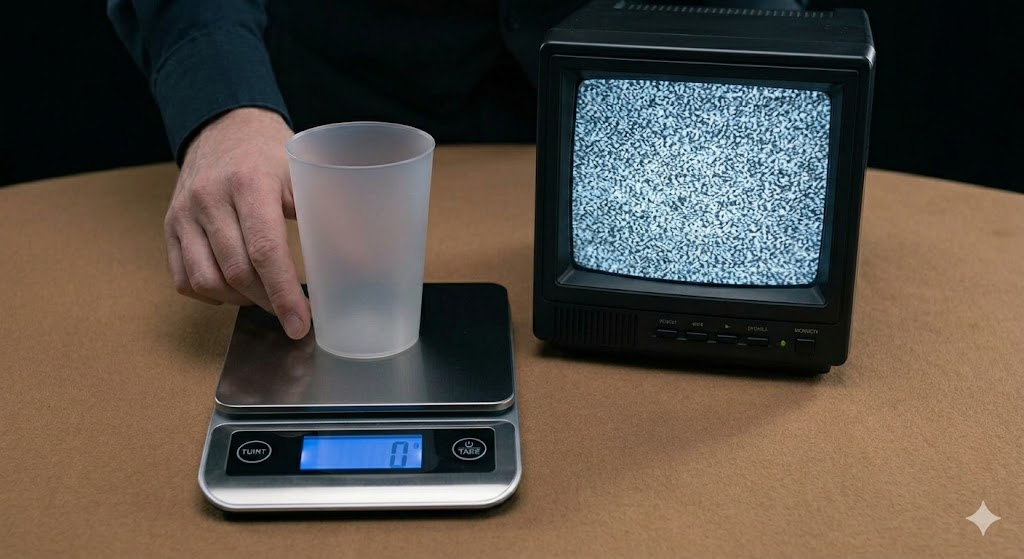
\includegraphics[keepaspectratio,alt={Figure 1}]{FIg1.jpeg}}
\caption{Figure 1}
\end{figure}

\begin{itemize}
\tightlist
\item
  \textbf{System (monitor):} static. Nothing (null). Only the inner wall
  of the cup.
\item
  \textbf{Observation (scale):} 0 g (the magician has zeroed / tared
  it).
\end{itemize}

\textbf{Mapping:} There is no subject to judge a state in the first
place. Hence \textbf{0 cannot be distinguished from null}. The scale's
zero, a concrete object, shows that ``nothing'' and ``zero'' look the
same. This does not mean 0 does not exist; it means it cannot be
distinguished from the interior.

\begin{center}\rule{0.5\linewidth}{0.5pt}\end{center}

\subsection{Figure 2: The first coin --- 1 indistinguishable from
0}\label{figure-2-the-first-coin-1-indistinguishable-from-0}

\begin{figure}
\centering
\pandocbounded{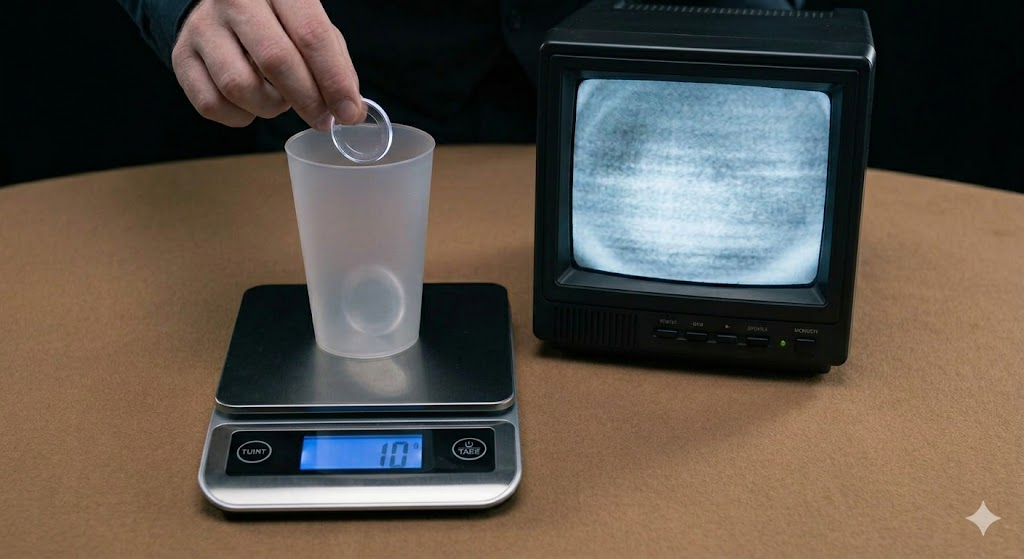
\includegraphics[keepaspectratio,alt={Figure 2}]{Fig2.jpeg}}
\caption{Figure 2}
\end{figure}

\begin{itemize}
\tightlist
\item
  \textbf{System (monitor):} almost no signal stands (only a faint
  blur). The sole coin's camera has \textbf{no ``other than itself'' to
  film}, and so cannot capture itself.
\item
  \textbf{Observation (scale):} 10 g. One coin is faintly visible in the
  cup.
\end{itemize}

\textbf{Mapping:} With no counterpart for comparison, the interior
cannot establish ``I exist.'' Hence \textbf{in the interior, 1 cannot be
distinguished from 0}. Meanwhile the scale (exterior) reads 10 g ---
\textbf{the exterior total has increased, yet no interior image stands}.
This discrepancy is the separation of interior and exterior itself.

\begin{center}\rule{0.5\linewidth}{0.5pt}\end{center}

\subsection{Figure 3: The second coin --- difference stands at
2}\label{figure-3-the-second-coin-difference-stands-at-2}

\begin{figure}
\centering
\pandocbounded{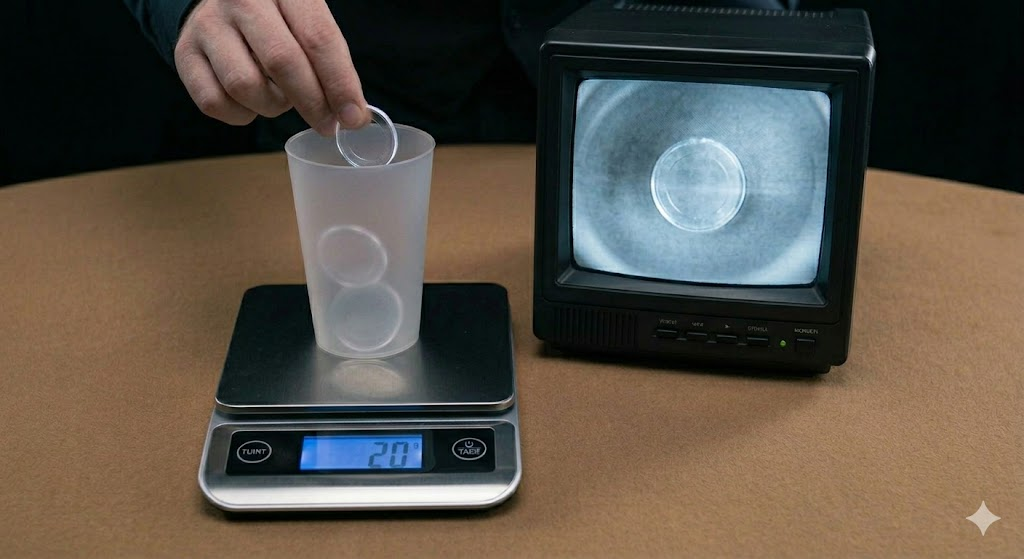
\includegraphics[keepaspectratio,alt={Figure 3}]{Fig3.jpeg}}
\caption{Figure 3}
\end{figure}

\begin{itemize}
\tightlist
\item
  \textbf{System (monitor):} for the first time, \textbf{ONE} clear
  transparent coin appears. One coin's camera has captured the other.
\item
  \textbf{Observation (scale):} 20 g. Two coins in the cup.
\end{itemize}

\textbf{Mapping:} For the first time ``an other than oneself'' appears,
and through it ``I exist'' stands. \textbf{Two is the minimum at which
anything can be known from the interior.} The ``one coin'' on the
monitor --- i.e., the first occurrence of ``1 (one other)'' in the
interior --- is the very birth of difference. Exterior (scale): 20 g;
interior (monitor): ``one other.''

\begin{center}\rule{0.5\linewidth}{0.5pt}\end{center}

\subsection{Figure 4: The third coin --- 2 and 2-or-more
indistinguishable (denial of hidden
variables)}\label{figure-4-the-third-coin-2-and-2-or-more-indistinguishable-denial-of-hidden-variables}

\begin{figure}
\centering
\pandocbounded{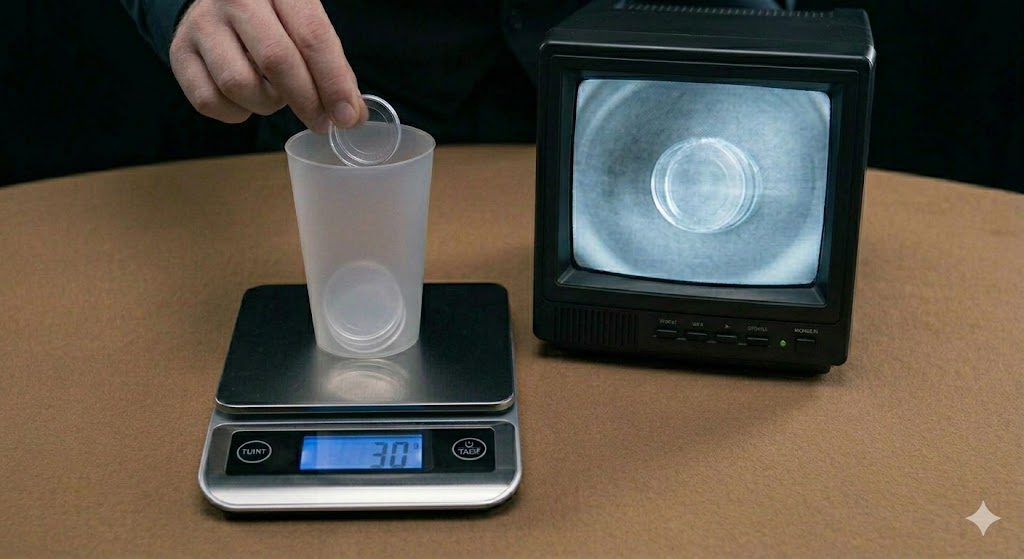
\includegraphics[keepaspectratio,alt={Figure 4}]{Fig4.jpeg}}
\caption{Figure 4}
\end{figure}

\begin{itemize}
\tightlist
\item
  \textbf{System (monitor):} still \textbf{ONE}. But on close inspection
  a \textbf{double edge (a doubled outline)} appears, the image slightly
  blurred. This is the trace of the magician's ``cheat'' --- stacking
  with a slight offset.
\item
  \textbf{Observation (scale):} 30 g. In the cup, an offset stack of
  coin shapes (a thick stack).
\end{itemize}

\textbf{Mapping:} The interior camera can film only up to ``an other is
present,'' and cannot separate whether that is 2 or 3. Hence \textbf{in
the interior, 2 and 2-or-more cannot be distinguished}. The double edge
is the only clue, but it is not information that fixes the count ---
\textbf{even shown everything from inside, it cannot be told}. This is
the \textbf{denial of hidden variables}: it is not that there is a
hidden variable ``the true count'' inside that is invisible due to
observational precision; rather, the interior viewpoint simply has no
structure to separate the count.

(The scale reads 30 g; as an additive conserved quantity, three units
stand. This is the objective exterior anchor and does not negate the
interior unknowability. \textbf{The exterior total can be read, but the
interior image cannot be counted} --- this asymmetry is the core of the
toy model.)

\begin{center}\rule{0.5\linewidth}{0.5pt}\end{center}

\subsection{Summary --- in one table}\label{summary-in-one-table}

{\def\LTcaptype{none} % do not increment counter
\begin{longtable}[]{@{}
  >{\raggedright\arraybackslash}p{(\linewidth - 6\tabcolsep) * \real{0.2500}}
  >{\raggedright\arraybackslash}p{(\linewidth - 6\tabcolsep) * \real{0.2500}}
  >{\raggedright\arraybackslash}p{(\linewidth - 6\tabcolsep) * \real{0.2500}}
  >{\raggedright\arraybackslash}p{(\linewidth - 6\tabcolsep) * \real{0.2500}}@{}}
\toprule\noalign{}
\begin{minipage}[b]{\linewidth}\raggedright
Fig
\end{minipage} & \begin{minipage}[b]{\linewidth}\raggedright
Scale (exterior / conserved)
\end{minipage} & \begin{minipage}[b]{\linewidth}\raggedright
Monitor (interior / unknowable)
\end{minipage} & \begin{minipage}[b]{\linewidth}\raggedright
What it shows
\end{minipage} \\
\midrule\noalign{}
\endhead
\bottomrule\noalign{}
\endlastfoot
1 & 0 g & null (static) & 0 and null cannot be distinguished \\
2 & 10 g & does not stand & 1 cannot be distinguished from 0 \\
3 & 20 g & one other, clear & difference stands at 2 (birth of ``1'' in
the interior) \\
4 & 30 g & one other (double edge) & 2 and 2-or-more cannot be
distinguished (denial of hidden variables) \\
\end{longtable}
}

While the exterior (scale) conserves and increases the quantity
additively as 0, 10, 20, 30, the interior (monitor) image saturates with
2 as its ceiling: \textbf{null → does not stand → one other → one other
(inseparable)}. The conserved total (exterior) can be counted; the
anonymous interior image cannot. The ``limit of anonymity = 2'' and
``interior unknowability does not negate the exterior integer
structure'' of §0.5 are reproduced right there on the table.

\begin{center}\rule{0.5\linewidth}{0.5pt}\end{center}

\subsection{Limitations of this model (reading
notes)}\label{limitations-of-this-model-reading-notes}

This note is not a rigorous proof but an \textbf{illustration} for
feeling the ontology of §0.5. As a toy model it involves
simplifications, and pushing for rigor only makes it harder to follow.
The following are notes to avoid misreading, not refinements of the
model.

\begin{enumerate}
\def\labelenumi{\arabic{enumi}.}
\item
  \textbf{The monitor is ``the first-person view of one anonymous
  element,''} not a god's-eye total. That is why, even with 2 coins, the
  screen shows only ``one other'' (from any one coin, only the single
  other is visible). The ``ONE'' in Figs. 3--4 is the image of ``an
  other has become present,'' not the interior starting to count.
\item
  \textbf{The scale reads only an additive total (a scalar), not ``the
  count.''} Obtaining ``3 coins'' from 30 g requires an \textbf{external
  assumption} that ``1 coin = 10 g and all are identical.'' That very
  identity is what anonymity does not license in the interior, so even
  the scale does not directly ``see'' the count. What stands objectively
  on the scale is the additive total, which does not contradict interior
  unknowability. The point of the toy model is the \textbf{asymmetry
  between interior unknowability and exterior total.}
\item
  \textbf{``Denial of hidden variables'' here is not in the sense of
  Bell's theorem.} It is distinct from the EPR/Bell no-hidden-variables
  result and is limited to the weak sense that ``the interior viewpoint
  simply has no structure to separate the count.''
\item
  \textbf{This toy model covers only part of §0.5.} It visualizes
  ``indistinguishability of 0, 1, 2'' and ``the absence of count
  separation''; the duality / conjugacy (``which of ν and λ is real
  cannot be asked'') is not included in the figures.
\item
  \textbf{No physical identification is made.} What the coins represent
  is not addressed.
\end{enumerate}

\begin{center}\rule{0.5\linewidth}{0.5pt}\end{center}

\subsection{Reference}\label{reference}

\begin{itemize}
\tightlist
\item
  Kihara, N. ``On the Logarithmic Map of Scale and the Separation of
  Scale and Quantization in a High-Symmetry Limit --- A Limited
  Verification Report from a Minimal Axiom System,'' §0.5. Concept DOI:
  \href{https://doi.org/10.5281/zenodo.20740841}{10.5281/zenodo.20740841};
  v1 DOI:
  \href{https://doi.org/10.5281/zenodo.20740842}{10.5281/zenodo.20740842}.
\end{itemize}
\end{document}
